\chapter{Approach and Implementation}
\label{chap:approach_and_implementation}

This chapter covers the various design approaches, flowchart of the approaches and methodology used in this work.

\section{Proposed Approach}
\label{sec:proposed_approach}
For Neural Architecture Search (NAS), various architectures needs to be explored and a method to encode this architecture is introduced in \autoref{sec:encoding_layers}. The concept of gene programming is used. While using NAS, the framework for the selection of the parents for mutation becomes essential. Along with the selection strategy, the method by which the mutation takes place also plays a vital role in generating new topologies that are efficient. In the following sections, we discuss the framework for the selection policies and the mutation strategy of generating new topologies. The fitness evaluation process is also discussed in the following sections.

\subsection{Encoding Layers}
\label{sec:encoding_layers}

Evolution is essential for using the NAS. For implementing the concept of evolution, this work uses genetic programming (gene expression programming). The architectures are represented by chromosomes that work as genotype and the set of architectures is referenced as the population. Parsing these chromosomes creates parse trees (or architecture tree as shown in Figure~\ref{fig:various_architecture}), which are called phenotype. A chromosome consists of a linear symbolic string of fixed length composed of genes of equal size. 

\begin{figure}[ht]
    \centering
    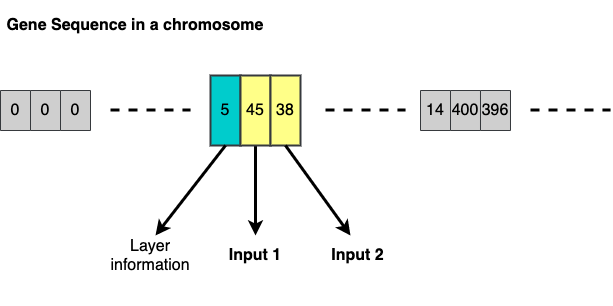
\includegraphics[width=1.0\linewidth, height=6cm]{BachelorMasterThesis/ApproachAndImplementation/Figures/gene_sequence.png}
    \caption{Example of a gene sequence}
    \label{fig:gene_sequence}
\end{figure}

Figure~\ref{fig:gene_sequence} shows a chromosome as a sequence of genes. Each gene is represented by an array of 3 numbers. The first number stores the information about the layer this gene is going to represent. The second and the third number stores the information about the layers from which this gene can receive the input from. If this layer can have multiple inputs, then both the numbers are used, else only the first number is used for the input. 

The number of genes in a chromosome can also be a variable. Also, all the genes are not active meaning that we don't use the entire gene sequence of the chromosome to form the network. Only the layers of the active genes are used to construct the network. We make use of two variables - one for the minimum number of active genes and one for the maximum number of active genes, to control the minimum and maximum number of layers in the network.

\subsection{Search space}
\label{sec:search_space}

The approach to create and explore the search space plays a vital role to find an optimal solution in NAS. The search space contains all feasible solutions which can lead to complications such as where to look for solutions to the problem, where to begin, or how to determine if a solution is the best solution.

Figure~\ref{fig:various_architecture} shows relatively simple architectures in which the layers of the neural networks are chained, in the sense that the architecture can be written as a sequence of n layers. Each node in the architecture corresponds to a layer of the neural network. Each edge represents the connection between two layers with the arrow providing the information about the input and output. 

\begin{figure}[t]
    \centering
    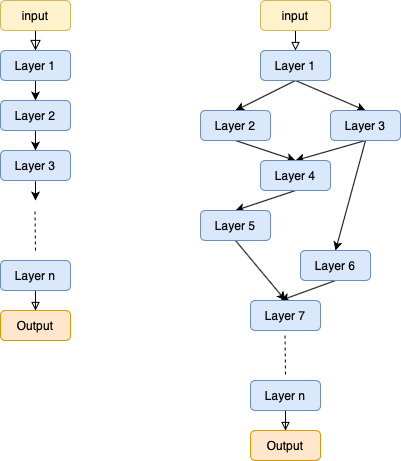
\includegraphics[width=0.7\linewidth, height=10cm]{BachelorMasterThesis/ApproachAndImplementation/Figures/VariousArchitecture.png}
    \caption{Illustration of various architecture}
    \label{fig:various_architecture}
\end{figure}

In the architecture on the left, the $i'th$ layer receives input from the $i - 1'th$ layer, resulting in a sequential model. The $i'th$ layer produces an output which serves as an input to the $i + 1'th$ layer. The architecture on the right is more complex as the $i'th$ layer can receive input from multiple previous layers. Also, the output from this layer can serve as an input to multiple layers, resulting in a non-sequential model.

In this work, convolutional layers, max-pooling, average pooling layers, sum, concatenation, and fully connected layers are used. The parameters to the convolutional layer are the filter size and kernel size with a stride size and padding size of '1' each. Particularly, this work uses filter size of $16,\: 32,\: 48$ and kernel size of $3 \; and \; 5$. The parameters to the pooling layers are the kernel of size $2 \; and \; 3$ and the stride of size $1 \;  and  \; 2$. To introduce a non-sequential element to the architectures, "sum" and "concatenation" layers with two inputs are used. Fully connected and average pooling layers are used as output layers.

The restrictions to the search space are added in the following way:
\begin{itemize}
    \item "n" number of layers : The number of layers is presently unbounded.
    \item The maximum and minimum number of parameters of an architecture are restricted to 100,000 and 4,000 respectively. This means that the number of parameters of a network cannot exceed 100,000 and cannot be less than 4,000.
    \item The architecture is evaluated for fitness before training. Only valid networks are trained after determining if each of the architecture path is valid. This also includes special checks for the concatenation and sum layer.
\end{itemize}

After introducing restrictions to search space, we use the principle of mutation to explore it. Mutation is part of the neuro-evolutionary method to explore search space. Evolutionary algorithms evolve a population of models. In every evolution step, at least one network (possibly trained) serves as a parent to generate offspring networks by applying mutation to the parent. Mutation, as mentioned in \autoref{sec:genetic_algorithm_background} involves altering a layer, either by making one of the gene inactive and making another gene active in the parent chromosome or modifying the layer information of one of the active gene. 

The mutation rate, a crucial hyperparameter, is used in the process of mutation of the parent. This parameter determines the variance of the configuration of the child from the parent. This essentially means that if a parent has a bad configuration, which is determined by the accuracy metric or a combination of accuracy, detection rate, false alarm rate and number of parameters, the child should be drastically different from the parent. This results in aggressive mutation for the child with a high mutation rate. But on the other hand, if the parent is a good network, then the child should only have small variations in the configuration with a low mutation rate. The mutation rate has a lower bound and an upper bound which adds variance in the process of mutation.

We use 3 kind of mutation in the work :

\begin{enumerate}
    \item \textbf{Random Mutation:} This kind of mutation is used to randomly mutate the genes of a network. Random, in this context, means changing the gene information by either activating/deactivating the gene or by modifying the layer information or by modifying the input layers to the gene. This mutation is only used when no previous network exists as this kind of mutation helps to generate new networks randomly. In this work, this mutation is only used to generate the initial population.
    \item \textbf{Genetic Mutation:} This kind of mutation is used to generate a child network from a parent network. This mutation is used when at least one previous network exists, that can be used as a parent. This kind of mutation helps to generate new networks by altering the genes of the parent network. If there are $\textbf{i}$ children to be generated in one generation, then this mutation creates a child - child[i] from a parent[i] i.e. the genes are mutated selectively from the parent network. In this work, except for the initial set of networks, all the other networks are generated using genetic mutation.
    \item \textbf{Neutral Mutation:} This kind of mutation is used to mutate the inactive genes of all parents for a generation. This mutation is used to enhance the gene diversity. This mutation is used to create a child network by only altering the inactive genes of a parent network. 
\end{enumerate}

An overall picture of the process of NAS implementation is explained in Figure~\ref{fig:nas_implementation}. This implementation is inspired by the work done by \cite{sun2020automatically}. As shown in the figure, initially, a certain number of random networks are generated with the restrictions to the search space mentioned above. This initial number is passed as a parameter from the command line. These networks belong to the set of initial population which are generated through random mutation. Also, the seed model (explained in \autoref{sec:seed_model}) can be added to the initial number of generated networks to improve the results. This first generation of the NAS process is then trained.

\begin{figure}[htbp]
    \centering
    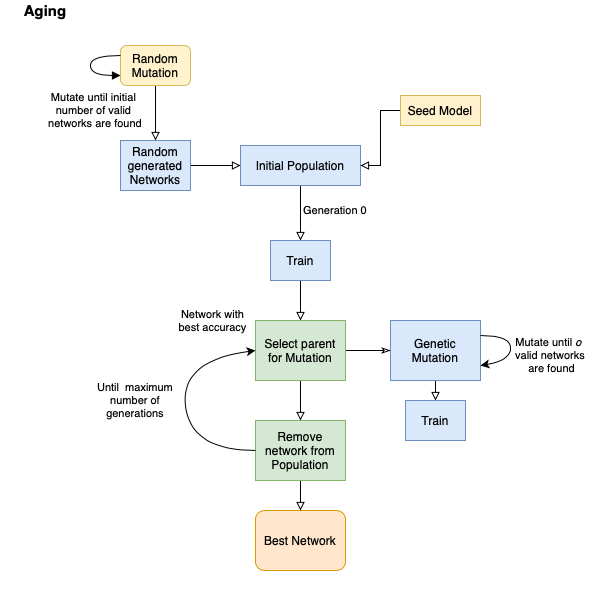
\includegraphics[width=1.0\linewidth, height=18cm]{BachelorMasterThesis/ApproachAndImplementation/Figures/Aging.png}
    \caption{Workflow of implementation of NAS}
    \label{fig:nas_implementation}
\end{figure}

\subsection{Fitness Evaluation}
\label{sec:fitness_evaluation}

All of the networks generated during the NAS process including the initial set of networks use the same input pipeline defined in~\autoref{sec:seed_model} for the training process. In figure~\ref{fig:nas_implementation}, this process is represented by the block "Train". Every network is associated with a network identifier and this is a counter that is incremented every time a new network is subjected to training. 
For the validation process, a custom validation function is added which uses the TFRecord for the validation dataset. Additionally custom values - detection rate and false alarm rate are added along with validation accuracy and validation loss. The values detection rate and false alarm rate are calculated based on true positive, true negative, false positive and false negative values. 

\begin{itemize}
    \item True positives - This is the count of the correctly predicted 'atrial fibrillation' labels by the model for the validation dataset. If the predicted label and the actual label is atrial fibrillation (which is value 1 in our work), then this counter is incremented by 1.
    \item True negatives - This is the count of the rightly predicted 'sinus rhythm' labels by the model for the validation dataset. If the predicted label and the actual label is sinus rhythm (which is value 0 in our work), then this counter is incremented by 1.
    \item False positives - This is the count of the falsely predicted 'atrial fibrillation' labels by the model for the validation dataset. If the predicted label is atrial fibrillation but the actual label is sinus rhythm (which is value 0 in our work), then this counter is incremented by 1.
    \item False negatives - This is the count of the falsely predicted 'sinus rhythm' labels by the model for the validation dataset. If the predicted label is sinus rhythm but the actual label is atrial fibrillation (which is value 1 in our work), then this counter is incremented by 1.
\end{itemize}

Based on the above four counters, detection rate and false alarm rate are calculated as follows:
\[ detection \; rate \; = \; true \; positives \; / \; (true \; positives \; + \; false \; negatives) \]
\[ false \; alarm \; rate \; = \; false \; positives \; / \; (false \; positives \; + \; true \; negatives) \]

In every generation, the first step is to select the fittest parents for mutation. This selection of parents is based on the selection strategy (explained in~\autoref{sec:selection_strategy}) and is represented by the block "Select parents for Mutation" in the figure~\ref{fig:nas_implementation}. After selecting the parents, the method of genetic mutation is used for generating children (or individuals). Again, depending on the selection strategy, either certain children or all of them are selected for training and trained in the manner described above. 

The next step is to select, among the newly trained children and the parents of this generation, those networks that are going to survive. These are the set of networks that are going to be used in the next generation for selecting a new set of parents. Along with this, the best network in this generation is also selected and stored in a variable. This network can be one of the newly trained children or one of the parents. We next look at the selection of parents for NAS.

\clearpage

\subsection{Selection strategy}
\label{sec:selection_strategy}

Evolutionary algorithms have a variety of methods to sample and select the parents for mutation and to generate offspring networks. This selection plays a significant role in exploring search space and producing good networks. In this project, there were four methods used to select the parent network. 

The selection policies are also used to train the offspring and select the networks to survive for the next generation among the entire population. The number of parents to be selected per generation is passed through the command line (we will use \textit{p} to represent this number). The other parameter used is the number of offspring to be generated at the end of each generation (we will use \textit{o} to represent this number). This parameter is also passed through the command line. For the selection strategy aging (described in the next section), this adds a condition that the initial population should be greater than the number of parents. 

Also, as one of the goal is to produce the smallest possible network with detection rate greater than 90\% and false alarm rate less than 20\%, we introduce a term called \textbf{weighted objectives}. This, along with accuracy are the measuring terms used in this thesis. Weighted objectives takes into account the number of parameters, the detection rate and the false alarm rate to calculate a weighted term which is then used for selecting the parent and the best network for the generation. The advantage of using this is that our definition of a good network is not based only on the accuracy, but also on the detection rate, false alarm rate and number of parameters. Essentially, if a network with less number of parameters produces good results, then such a network is more considered better for our scenario than a network with very high accuracy, but also with high number of parameters. 

The selection policies are explained in the following sections and are listed below:

\begin{enumerate}
    \item aging - This method trains all the children but the selection of a parent is random.
     \item all\_children - All offspring created from the parents are trained in every generation.
    \item selected\_children - Only selected offspring created from the parents are trained in every generation.
    \item lemonade - This method uses the concept of Pareto front. Pareto front optimizes multiple objectives such as accuracy and number of parameters.
\end{enumerate}

\subsubsection{Aging}

For the selection strategy of \textit{aging}, the logic for selection process is inspired from \cite{real2019regularized}. One of the goals of the selection process is to select a parent or parents for mutation. For \textit{aging}, at each cycle, from the set of available parents for mutation, \textit{p} networks are chosen at random, each drawn uniformly without replacement. As these networks are already trained, all the essential metrics such as accuracy, detection rate, etc. are available. From these networks, the network with either the best accuracy or with best weighted objectives is chosen as a parent for the mutation process.

The selection of the parent is followed by genetic mutation to mutate the parent to generate \textit{o} new networks. These are the offspring networks of this generation and are added to the current population. All these offspring are trained using the same pipeline mentioned above. The next phase of the NAS process is to eliminate a network or a set of networks from the current population. By this elimination process, we reduce the number of networks available for parent selection in the next generation.

For this strategy, the oldest network from the current population is eliminated (hence, the name aging). The remaining networks are available for parent selection in the next generation. This entire process is repeated for all the generations. 

The mutation of the parent provides exploration whereas parent selection provides exploitation. The parameter \textit{p} is used to control the aggressiveness of the exploitation process. Setting $\textit{p} \; = \; 1 $ reduces to random selection of parent and leading to random search. 

This selection strategy is used in evolutionary algorithms because of its simplicity. Although mutation causes a random construction of architecture thus rendering the entire process random, this strategy provides a distinctive advantage of mutating only the good models. Also, the NAS process is not affected significantly even if the best network is eliminated as the best available network is already mutated. Furthermore, by eliminating the oldest model, this strategy essentially favors the newer models in the population allowing us to explore the search space significantly rather than zeroing on the good models too early. Thus, this selection tends to improve the population over time.

\subsubsection{All\_children and selected\_children}

These selection policies are inspired by \cite{sun2020automatically}. For these strategies also, the first step is to select parent networks for mutation. The selection process for the first generation begins by selecting network identifiers as parents for mutation from the initial population. It is achieved by randomly creating \textit{o} number of pairs from \textit{p} available parents. Further, from all these pairs, the network with, either the better accuracy or with better weighted objectives is selected resulting in \textit{o} parents which can be used for mutation. An important note is that, because of the randomness of the creation of the pairs, there is the possibility that the same parent can be used for mutation multiple times. 

This is followed by genetic mutation to mutate \textit{o} available parents to create offspring for this generation. For the selection strategy \newline \textit{all\_children}, every offspring created from mutation is trained resulting in \textit{o} new networks every generation. For \textit{selected\_children}, a set of networks is selected randomly. This set can include parents from the previous generation and a subset of the offspring of this generation. Only the subset of the offspring are trained.

For both the selection policies, the next phase of the NAS process is to eliminate networks from the current population. This is achieved by pairwise comparison of networks according to the objectives. The pairs are created just before the training of the networks. Thus, after training, the same pairs are available with their essential metrics. The network with higher accuracy or better weighted objectives is chosen from the pair and is available for selection for the next generation. The remaining networks from the pairs are eliminated. This entire process is then repeated for all the generations.

\subsubsection{Lemonade and Pareto-front}

This selection strategy is inspired by \cite{elsken2018efficient}. Lemonade, as described by authors, is an evolutionary algorithm for multi-objective search with the search objectives in our case being the performance and the number of parameters of the model. This algorithm handles objectives separately categorizing them into cheap objectives (such as an architecture’s number of parameters) and expensive objectives (since it requires training the model first). The expensive objectives are the error rate, false alarm rate, and non-detection rate (1 - detection rate). 

The first step of the process is to determine candidates for mutation. The sampling of parents is done through a density function for the number of parameters (cheap objective). The density function searches for networks on the Pareto front where the network density is high. The next step is to generate \textit{o} new networks from the selected parents using genetic mutation. In the next stage, \textit{p} networks are chosen from \textit{o} networks based on the number of parameters, and these are trained and evaluated to obtain the results.

The final stage is to select networks which would survive for the next generation. A Pareto front is generated for the cheap objectives and expensive objectives. In every generation, the old Pareto front is combined with the children to generate a new Pareto front, and only those networks which lie on the Pareto front survive.

\subsubsection{Comparison of selection policies}

Every selection strategy has its advantages as well as disadvantages. The aging selection strategy is very easy to implement and has the advantage of generally mutating only good models. The population improves over time due to the removal of the oldest network but that might act as a disadvantage if run for a long period.

The selection policies - all\_children and selected\_children try to reduce the randomness by creating pairs and choosing the better network in the pair as parents. This improves the method used for the selection of parents in aging, which selects parents only randomly. Again, for the process of elimination, pairs are created for comparison, and a network with better accuracy or weighted objective is selected instead of removing the oldest network, which was the case in aging. This again improves the networks available for selection for the next generation. 

As selected\_children does not train all the children, there could be the case that a child that is created but not evaluated has a better accuracy than those trained. The strategy all\_children tries to explore more but requires a lot of training time as it tries to train all the created children.

In contrast, lemonade uses a Pareto-front strategy. Multiple objectives like error and number of parameters are optimized simultaneously. With this strategy, a set of networks is returned and it is up to the user to select a suitable network. The technique to optimize multiple objectives is an advantage for our use case. The final decision to select the network is taken by the user, for which the user needs to have a basic understanding of the use case. 

The results of all the above-mentioned selection policies are discussed in the next chapter.